\documentclass[border=10pt]{standalone}
\usepackage[svgnames]{xcolor}
\usepackage{amsmath}
\usepackage{pgfplots}
\pgfplotsset{compat=newest}
\usepackage[sfdefault]{FiraSans}
\usepackage{FiraMono}
\renewcommand*\familydefault{\sfdefault}
\begin{document}
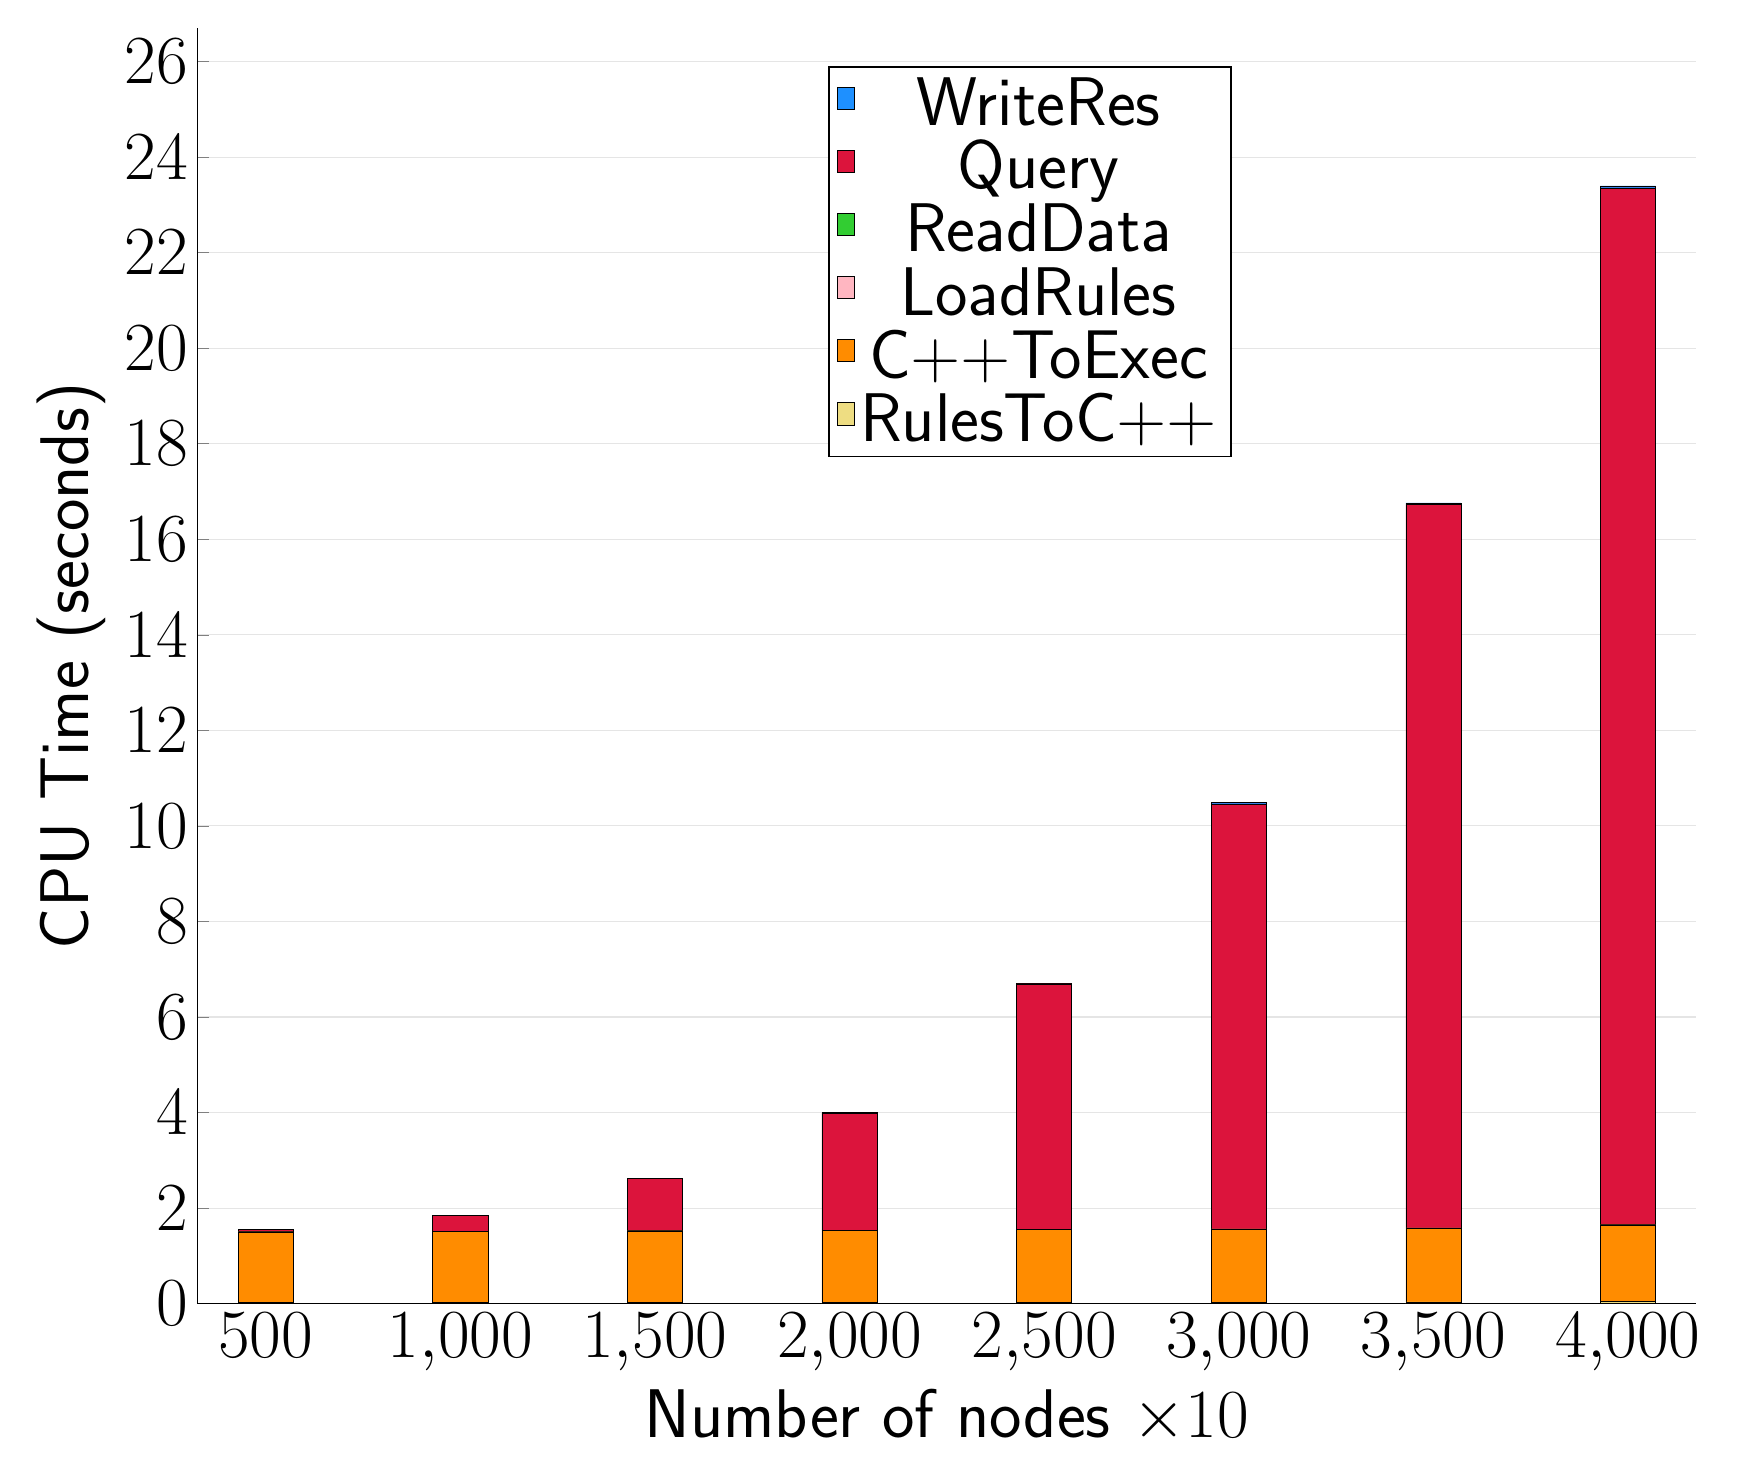
\begin{tikzpicture}
\begin{axis}[
   ybar stacked,
   width=1.7\textwidth,
   bar width=0.7cm,
   ymajorgrids, tick align=inside,
   major grid style={draw=gray!20},
   xtick=data,
   ymin=0, ymax=26.698890000000002,
   axis x line*=bottom,
   axis y line*=left,
   enlarge x limits=0.05,
   legend style={
       at={(0.69, 0.97)},
       anchor=north east,
       legend columns=1,
       font=\Huge,
   },
   ylabel={CPU Time (seconds)},
   xlabel={Number of nodes $\times 10$},
   label style={font=\Huge},
   tick label style={font=\Huge},
]
\addlegendimage{fill=DodgerBlue, draw=black, line width=0.2pt}
\addlegendentry{WriteRes}
\addlegendimage{fill=Crimson, draw=black, line width=0.2pt}
\addlegendentry{Query}
\addlegendimage{fill=LimeGreen, draw=black, line width=0.2pt}
\addlegendentry{ReadData}
\addlegendimage{fill=LightPink, draw=black, line width=0.2pt}
\addlegendentry{LoadRules}
\addlegendimage{fill=DarkOrange, draw=black, line width=0.2pt}
\addlegendentry{C++ToExec}
\addlegendimage{fill=LightGoldenrod, draw=black, line width=0.2pt}
\addlegendentry{RulesToC++}
\addplot +[fill=LightGoldenrod, draw=black, line width=0.2pt] coordinates {
(500, 0.030000000000000006)
(1000, 0.030000000000000006)
(1500, 0.030000000000000006)
(2000, 0.030000000000000006)
(2500, 0.031000000000000007)
(3000, 0.031000000000000007)
(3500, 0.036)
(4000, 0.041999999999999996)
};
\addplot +[fill=DarkOrange, draw=black, line width=0.2pt] coordinates {
(500, 1.473)
(1000, 1.4760000000000002)
(1500, 1.4920000000000002)
(2000, 1.504)
(2500, 1.5240000000000002)
(3000, 1.525)
(3500, 1.539)
(4000, 1.605)
};
\addplot +[fill=LightPink, draw=black, line width=0.2pt] coordinates {
(500, 9.609999999999999e-05)
(1000, 8.65e-05)
(1500, 6.63e-05)
(2000, 3.33e-05)
(2500, 5.22e-05)
(3000, 0.0001088)
(3500, 9.77e-05)
(4000, 6.45e-05)
};
\addplot +[fill=LimeGreen, draw=black, line width=0.2pt] coordinates {
(500, 0.0014632)
(1000, 0.0026191)
(1500, 0.0035453)
(2000, 0.0044359)
(2500, 0.005587399999999999)
(3000, 0.0064504)
(3500, 0.0079138)
(4000, 0.008193200000000001)
};
\addplot +[fill=Crimson, draw=black, line width=0.2pt] coordinates {
(500, 0.0535867)
(1000, 0.3307171)
(1500, 1.095862)
(2000, 2.450427)
(2500, 5.131427)
(3000, 8.899659)
(3500, 15.14585)
(4000, 21.698890000000002)
};
\addplot +[fill=DodgerBlue, draw=black, line width=0.2pt] coordinates {
(500, 0.0009061)
(1000, 0.0029717)
(1500, 0.0065487)
(2000, 0.011430899999999999)
(2500, 0.017599999999999998)
(3000, 0.025351999999999996)
(3500, 0.034351900000000005)
(4000, 0.04497399999999999)
};
\end{axis}
\end{tikzpicture}

\end{document}
